\chapter{Two Processors}
\label{chap:p2}

\section{Another recursion describing optimal expected run time}
\label{sec:p2-simple-method-for-runtime}

\newcommand{\profile}[1]{\left\llbracket #1 \right\rrbracket}

If one considers the problem of scheduling an intree onto two processors, it becomes clear that HLF is optimal (\todo{Proof.}). \todo{Is the following correct:} Moreover, we can conclude that we can compute the optimal expected finish time in polynomial time.

This section shows how the original problem of an intree DAG can be mapped onto another, more compact structure.

\subsection{Profiles of Intrees}
\label{sec:p2-simple-method-runtime-profiles-for-intrees}

If we consider the trees in figure \ref{fig:p2-four-intrees-with-same-profile-6-3-1}, we can compute that for two processors HLF always yields an expected run time of $\frac{49}{8}$ for each of them, which is optimal:

\begin{figure}[ht]
  \centering
  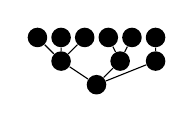
\begin{tikzpicture}[scale=.2]
\node[circle, scale=0.75, fill] (tid0) at (4.5,1.5){};
\node[circle, scale=0.75, fill] (tid1) at (2.25,3){};
\node[circle, scale=0.75, fill] (tid4) at (0.75,4.5){};
\node[circle, scale=0.75, fill] (tid5) at (2.25,4.5){};
\node[circle, scale=0.75, fill] (tid6) at (3.75,4.5){};
\draw[](tid1) -- (tid4);
\draw[](tid1) -- (tid5);
\draw[](tid1) -- (tid6);
\node[circle, scale=0.75, fill] (tid2) at (6,3){};
\node[circle, scale=0.75, fill] (tid7) at (5.25,4.5){};
\node[circle, scale=0.75, fill] (tid8) at (6.75,4.5){};
\draw[](tid2) -- (tid7);
\draw[](tid2) -- (tid8);
\node[circle, scale=0.75, fill] (tid3) at (8.25,3){};
\node[circle, scale=0.75, fill] (tid9) at (8.25,4.5){};
\draw[](tid3) -- (tid9);
\draw[](tid0) -- (tid1);
\draw[](tid0) -- (tid2);
\draw[](tid0) -- (tid3);
\end{tikzpicture}
%%% Local Variables:
%%% TeX-master: "thesis/thesis.tex"
%%% End: \hspace{0.5cm}
  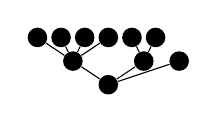
\begin{tikzpicture}[scale=.2]
\node[circle, scale=0.75, fill] (tid0) at (5.25,1.5){};
\node[circle, scale=0.75, fill] (tid1) at (3,3){};
\node[circle, scale=0.75, fill] (tid4) at (0.75,4.5){};
\node[circle, scale=0.75, fill] (tid5) at (2.25,4.5){};
\node[circle, scale=0.75, fill] (tid6) at (3.75,4.5){};
\node[circle, scale=0.75, fill] (tid7) at (5.25,4.5){};
\draw[](tid1) -- (tid4);
\draw[](tid1) -- (tid5);
\draw[](tid1) -- (tid6);
\draw[](tid1) -- (tid7);
\node[circle, scale=0.75, fill] (tid2) at (7.5,3){};
\node[circle, scale=0.75, fill] (tid8) at (6.75,4.5){};
\node[circle, scale=0.75, fill] (tid9) at (8.25,4.5){};
\draw[](tid2) -- (tid8);
\draw[](tid2) -- (tid9);
\node[circle, scale=0.75, fill] (tid3) at (9.75,3){};
\draw[](tid0) -- (tid1);
\draw[](tid0) -- (tid2);
\draw[](tid0) -- (tid3);
\end{tikzpicture}
%%% Local Variables:
%%% TeX-master: "thesis/thesis.tex"
%%% End: \hspace{0.5cm}
  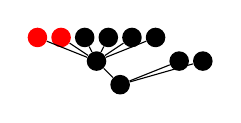
\begin{tikzpicture}[scale=.2]
\node[circle, scale=0.75, fill] (tid0) at (6,1.5){};
\node[circle, scale=0.75, fill] (tid1) at (4.5,3){};
\node[circle, scale=0.75, fill, red] (tid4) at (0.75,4.5){};
\node[circle, scale=0.75, fill, red] (tid5) at (2.25,4.5){};
\node[circle, scale=0.75, fill] (tid6) at (3.75,4.5){};
\node[circle, scale=0.75, fill] (tid7) at (5.25,4.5){};
\node[circle, scale=0.75, fill] (tid8) at (6.75,4.5){};
\node[circle, scale=0.75, fill] (tid9) at (8.25,4.5){};
\draw[](tid1) -- (tid4);
\draw[](tid1) -- (tid5);
\draw[](tid1) -- (tid6);
\draw[](tid1) -- (tid7);
\draw[](tid1) -- (tid8);
\draw[](tid1) -- (tid9);
\node[circle, scale=0.75, fill] (tid2) at (9.75,3){};
\node[circle, scale=0.75, fill] (tid3) at (11.25,3){};
\draw[](tid0) -- (tid1);
\draw[](tid0) -- (tid2);
\draw[](tid0) -- (tid3);
\end{tikzpicture}
%%% Local Variables:
%%% TeX-master: "thesis/thesis.tex"
%%% End: \hspace{0.5cm}
  \begin{tikzpicture}[scale=.2]
\node[circle, scale=0.75, fill] (tid0) at (5.25,1.5){};
\node[circle, scale=0.75, fill] (tid1) at (2.25,3){};
\node[circle, scale=0.75, fill, task_scheduled] (tid4) at (0.75,4.5){};
\node[circle, scale=0.75, fill] (tid5) at (2.25,4.5){};
\node[circle, scale=0.75, fill] (tid6) at (3.75,4.5){};
\draw[](tid1) -- (tid4);
\draw[](tid1) -- (tid5);
\draw[](tid1) -- (tid6);
\node[circle, scale=0.75, fill] (tid2) at (6.75,3){};
\node[circle, scale=0.75, fill, task_scheduled] (tid7) at (5.25,4.5){};
\node[circle, scale=0.75, fill] (tid8) at (6.75,4.5){};
\node[circle, scale=0.75, fill] (tid9) at (8.25,4.5){};
\draw[](tid2) -- (tid7);
\draw[](tid2) -- (tid8);
\draw[](tid2) -- (tid9);
\node[circle, scale=0.75, fill] (tid3) at (9.75,3){};
\draw[](tid0) -- (tid1);
\draw[](tid0) -- (tid2);
\draw[](tid0) -- (tid3);
\end{tikzpicture}
%%% Local Variables:
%%% TeX-master: "thesis/thesis.tex"
%%% End: 
  \caption{Four intrees with the same profile ($\profile{6,3,1}$). All of them have expected run time of $49/8$ if scheduled with HLF on two processors.}
  \label{fig:p2-four-intrees-with-same-profile-6-3-1}
\end{figure}

The intrees in figure \ref{fig:p2-four-intrees-with-same-profile-6-3-1} have the following in common: At each level, they have the same amount of tasks (six tasks at the topmost level, three in the middle one and one at the bottom level).

We can use the number of tasks per level as a (non-bijective) ``encoding'' of intrees. For now, we call this encoding a \emph{profile} of the intree. The above intrees would all be encoded as a profile containing the numbers 6, 3 and 1 in that order. We denote the profile by $\profile{6, 3, 1}$.

Note that not all sequences of numbers can be used as profiles. In particular, the last number in a profile is (w.l.o.g.) 1 (since we have only one task as the root of the tree)\footnote{This, of course, introduces some overhead in notation, but we leave it as it is since it is easier to read this way.}. Moreover, it can not be the case that there is a zero in a profile (since this would imply that there is \emph{no task} on one specific level in the intree).

\subsection{Profiles and HLF}
\label{sec:p2-simple-method-runtime-profiles-hlf}

For two processors and HLF-scheduling, we can easily conclude the successors of a profile. Let us first of all consider some examples here: If we have the profile $\profile{5,4,2,1}$, then two of the five topmost tasks \emph{have to be scheduled} (since we are using HLF). If one of these two topmost tasks is finished, we reach $\profile{4,4,2,1}$ (see figure \ref{fig:p2-profiles-successors-of-5421-always-same} for reference).

\begin{figure}[ht]
  \centering
  \renewcommand{\leveltopI}{-10cm + \leveltop}
\renewcommand{\leveltopII}{-10cm + \leveltopI}
\renewcommand{\leveltopIII}{-10cm + \leveltopII}
\renewcommand{\leveltopIIII}{-10cm + \leveltopIII}
\renewcommand{\leveltopIIIII}{-10cm + \leveltopIIII}
\renewcommand{\leveltopIIIIII}{-10cm + \leveltopIIIII}
\renewcommand{\leveltopIIIIIII}{-10cm + \leveltopIIIIII}
\renewcommand{\leveltopIIIIIIII}{-10cm + \leveltopIIIIIII}
\renewcommand{\leveltopIIIIIIIII}{-10cm + \leveltopIIIIIIII}
\renewcommand{\leveltopIIIIIIIIII}{-10cm + \leveltopIIIIIIIII}
\renewcommand{\leveltopIIIIIIIIIII}{-10cm + \leveltopIIIIIIIIII}
\renewcommand{\leveltopIIIIIIIIIIII}{-10cm + \leveltopIIIIIIIIIII}
\renewcommand{\leveltopI}{-10cm + \leveltop}
\renewcommand{\leveltopII}{-10cm + \leveltopI}
\renewcommand{\leveltopIII}{-10cm + \leveltopII}
\renewcommand{\leveltopIIII}{-10cm + \leveltopIII}
\renewcommand{\leveltopIIIII}{-10cm + \leveltopIIII}
\renewcommand{\leveltopIIIIII}{-10cm + \leveltopIIIII}
\renewcommand{\leveltopIIIIIII}{-10cm + \leveltopIIIIII}
\renewcommand{\leveltopIIIIIIII}{-10cm + \leveltopIIIIIII}
\renewcommand{\leveltopIIIIIIIII}{-10cm + \leveltopIIIIIIII}
\renewcommand{\leveltopIIIIIIIIII}{-10cm + \leveltopIIIIIIIII}
\renewcommand{\leveltopIIIIIIIIIII}{-10cm + \leveltopIIIIIIIIII}
\renewcommand{\leveltopIIIIIIIIIIII}{-10cm + \leveltopIIIIIIIIIII}
\begin{tikzpicture}[scale=.2, anchor=south]
\begin{scope}[yshift=\leveltopI cm]
\matrix (line1)[column sep=0.1cm] {
\node[draw=black, rectangle split,  rectangle split parts=1] (sn0x9b5d5c8){
\begin{tikzpicture}[scale=.2]
\node[circle, scale=0.75, fill] (tid0) at (4.5,1.5){};
\node[circle, scale=0.75, fill] (tid1) at (3,3){};
\node[circle, scale=0.75, fill] (tid3) at (1.5,4.5){};
\node[circle, scale=0.75, fill, task_scheduled] (tid7) at (0.75,6){};
\node[circle, scale=0.75, fill, task_scheduled] (tid8) at (2.25,6){};
\draw[](tid3) -- (tid7);
\draw[](tid3) -- (tid8);
\node[circle, scale=0.75, fill] (tid4) at (3.75,4.5){};
\node[circle, scale=0.75, fill] (tid9) at (3.75,6){};
\draw[](tid4) -- (tid9);
\node[circle, scale=0.75, fill] (tid5) at (5.25,4.5){};
\draw[](tid1) -- (tid3);
\draw[](tid1) -- (tid4);
\draw[](tid1) -- (tid5);
\node[circle, scale=0.75, fill] (tid2) at (7.5,3){};
\node[circle, scale=0.75, fill] (tid6) at (7.5,4.5){};
\node[circle, scale=0.75, fill] (tid10) at (6.75,6){};
\node[circle, scale=0.75, fill] (tid11) at (8.25,6){};
\draw[](tid6) -- (tid10);
\draw[](tid6) -- (tid11);
\draw[](tid2) -- (tid6);
\draw[](tid0) -- (tid1);
\draw[](tid0) -- (tid2);
\end{tikzpicture}
};
 & 
\\
};
\end{scope}
\begin{scope}[yshift=\leveltopII cm]
\matrix (line2)[column sep=0.1cm] {
\node[draw=black, rectangle split,  rectangle split parts=1] (sn0x9b5de08){
\begin{tikzpicture}[scale=.2]
\node[circle, scale=0.75, fill] (tid0) at (3.75,1.5){};
\node[circle, scale=0.75, fill] (tid1) at (2.25,3){};
\node[circle, scale=0.75, fill] (tid3) at (0.75,4.5){};
\node[circle, scale=0.75, fill, task_scheduled] (tid7) at (0.75,6){};
\draw[](tid3) -- (tid7);
\node[circle, scale=0.75, fill] (tid4) at (2.25,4.5){};
\node[circle, scale=0.75, fill, task_scheduled] (tid8) at (2.25,6){};
\draw[](tid4) -- (tid8);
\node[circle, scale=0.75, fill] (tid5) at (3.75,4.5){};
\draw[](tid1) -- (tid3);
\draw[](tid1) -- (tid4);
\draw[](tid1) -- (tid5);
\node[circle, scale=0.75, fill] (tid2) at (6,3){};
\node[circle, scale=0.75, fill] (tid6) at (6,4.5){};
\node[circle, scale=0.75, fill] (tid9) at (5.25,6){};
\node[circle, scale=0.75, fill] (tid10) at (6.75,6){};
\draw[](tid6) -- (tid9);
\draw[](tid6) -- (tid10);
\draw[](tid2) -- (tid6);
\draw[](tid0) -- (tid1);
\draw[](tid0) -- (tid2);
\end{tikzpicture}
};
 & 
\node[draw=black, rectangle split,  rectangle split parts=1] (sn0x9b58978){
\begin{tikzpicture}[scale=.2]
\node[circle, scale=0.75, fill] (tid0) at (3.75,1.5){};
\node[circle, scale=0.75, fill] (tid1) at (2.25,3){};
\node[circle, scale=0.75, fill] (tid3) at (0.75,4.5){};
\node[circle, scale=0.75, fill, task_scheduled] (tid7) at (0.75,6){};
\draw[](tid3) -- (tid7);
\node[circle, scale=0.75, fill] (tid4) at (2.25,4.5){};
\node[circle, scale=0.75, fill] (tid8) at (2.25,6){};
\draw[](tid4) -- (tid8);
\node[circle, scale=0.75, fill] (tid5) at (3.75,4.5){};
\draw[](tid1) -- (tid3);
\draw[](tid1) -- (tid4);
\draw[](tid1) -- (tid5);
\node[circle, scale=0.75, fill] (tid2) at (6,3){};
\node[circle, scale=0.75, fill] (tid6) at (6,4.5){};
\node[circle, scale=0.75, fill, task_scheduled] (tid9) at (5.25,6){};
\node[circle, scale=0.75, fill] (tid10) at (6.75,6){};
\draw[](tid6) -- (tid9);
\draw[](tid6) -- (tid10);
\draw[](tid2) -- (tid6);
\draw[](tid0) -- (tid1);
\draw[](tid0) -- (tid2);
\end{tikzpicture}
};
 & 
\\
};
\end{scope}
\draw (sn0x9b5d5c8.south) -- (sn0x9b5de08.north);
\draw (sn0x9b5d5c8.south) -- (sn0x9b58978.north);
\end{tikzpicture}
\renewcommand{\leveltopI}{-10cm + \leveltop}
\renewcommand{\leveltopII}{-10cm + \leveltopI}
\renewcommand{\leveltopIII}{-10cm + \leveltopII}
\renewcommand{\leveltopIIII}{-10cm + \leveltopIII}
\renewcommand{\leveltopIIIII}{-10cm + \leveltopIIII}
\renewcommand{\leveltopIIIIII}{-10cm + \leveltopIIIII}
\renewcommand{\leveltopIIIIIII}{-10cm + \leveltopIIIIII}
\renewcommand{\leveltopIIIIIIII}{-10cm + \leveltopIIIIIII}
\renewcommand{\leveltopIIIIIIIII}{-10cm + \leveltopIIIIIIII}
\renewcommand{\leveltopIIIIIIIIII}{-10cm + \leveltopIIIIIIIII}
\renewcommand{\leveltopIIIIIIIIIII}{-10cm + \leveltopIIIIIIIIII}
\renewcommand{\leveltopIIIIIIIIIIII}{-10cm + \leveltopIIIIIIIIIII}
\begin{tikzpicture}[scale=.2, anchor=south]
\begin{scope}[yshift=\leveltopI cm]
\matrix (line1)[column sep=0.1cm] {
\node[draw=black, rectangle split,  rectangle split parts=1] (sn0x9b5ed70){
\begin{tikzpicture}[scale=.2]
\node[circle, scale=0.75, fill] (tid0) at (4.5,1.5){};
\node[circle, scale=0.75, fill] (tid1) at (3,3){};
\node[circle, scale=0.75, fill] (tid3) at (1.5,4.5){};
\node[circle, scale=0.75, fill, task_scheduled] (tid7) at (0.75,6){};
\node[circle, scale=0.75, fill] (tid8) at (2.25,6){};
\draw[](tid3) -- (tid7);
\draw[](tid3) -- (tid8);
\node[circle, scale=0.75, fill] (tid4) at (3.75,4.5){};
\node[circle, scale=0.75, fill, task_scheduled] (tid9) at (3.75,6){};
\draw[](tid4) -- (tid9);
\node[circle, scale=0.75, fill] (tid5) at (5.25,4.5){};
\draw[](tid1) -- (tid3);
\draw[](tid1) -- (tid4);
\draw[](tid1) -- (tid5);
\node[circle, scale=0.75, fill] (tid2) at (7.5,3){};
\node[circle, scale=0.75, fill] (tid6) at (7.5,4.5){};
\node[circle, scale=0.75, fill] (tid10) at (6.75,6){};
\node[circle, scale=0.75, fill] (tid11) at (8.25,6){};
\draw[](tid6) -- (tid10);
\draw[](tid6) -- (tid11);
\draw[](tid2) -- (tid6);
\draw[](tid0) -- (tid1);
\draw[](tid0) -- (tid2);
\end{tikzpicture}
};
 & 
\\
};
\end{scope}
\begin{scope}[yshift=\leveltopII cm]
\matrix (line2)[column sep=0.1cm] {
\node[draw=black, rectangle split,  rectangle split parts=1] (sn0x9b5e2b0){
\begin{tikzpicture}[scale=.2]
\node[circle, scale=0.75, fill] (tid0) at (4.5,1.5){};
\node[circle, scale=0.75, fill] (tid1) at (3,3){};
\node[circle, scale=0.75, fill] (tid3) at (1.5,4.5){};
\node[circle, scale=0.75, fill, task_scheduled] (tid7) at (0.75,6){};
\node[circle, scale=0.75, fill, task_scheduled] (tid8) at (2.25,6){};
\draw[](tid3) -- (tid7);
\draw[](tid3) -- (tid8);
\node[circle, scale=0.75, fill] (tid4) at (3.75,4.5){};
\node[circle, scale=0.75, fill] (tid5) at (5.25,4.5){};
\draw[](tid1) -- (tid3);
\draw[](tid1) -- (tid4);
\draw[](tid1) -- (tid5);
\node[circle, scale=0.75, fill] (tid2) at (7.5,3){};
\node[circle, scale=0.75, fill] (tid6) at (7.5,4.5){};
\node[circle, scale=0.75, fill] (tid9) at (6.75,6){};
\node[circle, scale=0.75, fill] (tid10) at (8.25,6){};
\draw[](tid6) -- (tid9);
\draw[](tid6) -- (tid10);
\draw[](tid2) -- (tid6);
\draw[](tid0) -- (tid1);
\draw[](tid0) -- (tid2);
\end{tikzpicture}
};
 & 
\node[draw=black, rectangle split,  rectangle split parts=1] (sn0x9b5ebe0){
\begin{tikzpicture}[scale=.2]
\node[circle, scale=0.75, fill] (tid0) at (4.5,1.5){};
\node[circle, scale=0.75, fill] (tid1) at (3,3){};
\node[circle, scale=0.75, fill] (tid3) at (1.5,4.5){};
\node[circle, scale=0.75, fill, task_scheduled] (tid7) at (0.75,6){};
\node[circle, scale=0.75, fill] (tid8) at (2.25,6){};
\draw[](tid3) -- (tid7);
\draw[](tid3) -- (tid8);
\node[circle, scale=0.75, fill] (tid4) at (3.75,4.5){};
\node[circle, scale=0.75, fill] (tid5) at (5.25,4.5){};
\draw[](tid1) -- (tid3);
\draw[](tid1) -- (tid4);
\draw[](tid1) -- (tid5);
\node[circle, scale=0.75, fill] (tid2) at (7.5,3){};
\node[circle, scale=0.75, fill] (tid6) at (7.5,4.5){};
\node[circle, scale=0.75, fill, task_scheduled] (tid9) at (6.75,6){};
\node[circle, scale=0.75, fill] (tid10) at (8.25,6){};
\draw[](tid6) -- (tid9);
\draw[](tid6) -- (tid10);
\draw[](tid2) -- (tid6);
\draw[](tid0) -- (tid1);
\draw[](tid0) -- (tid2);
\end{tikzpicture}
};
 & 
\node[draw=black, rectangle split,  rectangle split parts=1] (sn0x9b5de08){
\begin{tikzpicture}[scale=.2]
\node[circle, scale=0.75, fill] (tid0) at (3.75,1.5){};
\node[circle, scale=0.75, fill] (tid1) at (2.25,3){};
\node[circle, scale=0.75, fill] (tid3) at (0.75,4.5){};
\node[circle, scale=0.75, fill, task_scheduled] (tid7) at (0.75,6){};
\draw[](tid3) -- (tid7);
\node[circle, scale=0.75, fill] (tid4) at (2.25,4.5){};
\node[circle, scale=0.75, fill, task_scheduled] (tid8) at (2.25,6){};
\draw[](tid4) -- (tid8);
\node[circle, scale=0.75, fill] (tid5) at (3.75,4.5){};
\draw[](tid1) -- (tid3);
\draw[](tid1) -- (tid4);
\draw[](tid1) -- (tid5);
\node[circle, scale=0.75, fill] (tid2) at (6,3){};
\node[circle, scale=0.75, fill] (tid6) at (6,4.5){};
\node[circle, scale=0.75, fill] (tid9) at (5.25,6){};
\node[circle, scale=0.75, fill] (tid10) at (6.75,6){};
\draw[](tid6) -- (tid9);
\draw[](tid6) -- (tid10);
\draw[](tid2) -- (tid6);
\draw[](tid0) -- (tid1);
\draw[](tid0) -- (tid2);
\end{tikzpicture}
};
 & 
\node[draw=black, rectangle split,  rectangle split parts=1] (sn0x9b58978){
\begin{tikzpicture}[scale=.2]
\node[circle, scale=0.75, fill] (tid0) at (3.75,1.5){};
\node[circle, scale=0.75, fill] (tid1) at (2.25,3){};
\node[circle, scale=0.75, fill] (tid3) at (0.75,4.5){};
\node[circle, scale=0.75, fill, task_scheduled] (tid7) at (0.75,6){};
\draw[](tid3) -- (tid7);
\node[circle, scale=0.75, fill] (tid4) at (2.25,4.5){};
\node[circle, scale=0.75, fill] (tid8) at (2.25,6){};
\draw[](tid4) -- (tid8);
\node[circle, scale=0.75, fill] (tid5) at (3.75,4.5){};
\draw[](tid1) -- (tid3);
\draw[](tid1) -- (tid4);
\draw[](tid1) -- (tid5);
\node[circle, scale=0.75, fill] (tid2) at (6,3){};
\node[circle, scale=0.75, fill] (tid6) at (6,4.5){};
\node[circle, scale=0.75, fill, task_scheduled] (tid9) at (5.25,6){};
\node[circle, scale=0.75, fill] (tid10) at (6.75,6){};
\draw[](tid6) -- (tid9);
\draw[](tid6) -- (tid10);
\draw[](tid2) -- (tid6);
\draw[](tid0) -- (tid1);
\draw[](tid0) -- (tid2);
\end{tikzpicture}
};
 & 
\\
};
\end{scope}
\draw (sn0x9b5ed70.south) -- (sn0x9b5e2b0.north);
\draw (sn0x9b5ed70.south) -- (sn0x9b5ebe0.north);
\draw (sn0x9b5ed70.south) -- (sn0x9b5de08.north);
\draw (sn0x9b5ed70.south) -- (sn0x9b58978.north);
\end{tikzpicture}
%%% Local Variables:
%%% TeX-master: "thesis/thesis.tex"
%%% End: 

  \caption{Intree with profile $\profile{5,4,2,1}$. \emph{All} possible HLF-successors of the original intree have profile $\profile{4,4,2,1}$.}
  \label{fig:p2-profiles-successors-of-5421-always-same}
\end{figure}

\todo{More figures.}

Another interesting case is $\profile{1,5,2,1}$, where the (single) topmost task and one of the five tasks on the second level are scheduled. If the topmost task is finished (which happens with probability $\frac{1}{2}$), we reach $\profile{5,2,1}$. If the scheduled task on the second level finishes first, we reach $\profile{1,4,2,1}$.

The last example we want to give here is $\profile{1,1,1,3,1}$. In this case, the single topmost task and one of the three tasks of the second lowest level have to be scheduled. If the topmost task finishes first (which happens with probability $\frac{1}{2}$), the resulting profile will be $\profile{1,1,3,1}$ (where again the topmost task and one of the tree tasks in the second lowest level are scheduled). If the other scheduled task finishes first, we reach $\profile{1,1,1,2,1}$, where the single topmost task and one of the remaining \emph{two} tasks on the second lowest level are scheduled.

We now use the profile notation to denote the expected run time (i.e. we say $\profile{6,3,1} = \frac{49}{8}$ --- see figure \ref{fig:p2-four-intrees-with-same-profile-6-3-1}).

Exploiting this notation, we can define the following recursive formula that can be used to compute the optimal expected run time:

\begin{equation}
  \label{eq:p2-profile-optimal-exp-run-time}
  \profile{n_1, \dots, n_r} =
  \begin{cases}
    r, & \text{ if } n_1 = n_2 = \dots = n_r = 1 \\
    \frac{n_1-1}{2} + \profile{1, n_2, n_3, \dots, n_r} , & \text{ if } n_r\geq 2 \\
    \frac{1}{2} + \frac{1}{2} \cdot \left( \profile{n_2, \dots, n_r} + SUC(\profile{n_1,\dots,n_r}) \right) ,& \text{ otherwise }
  \end{cases},
\end{equation}
where $SUC(\profile{n_1,\dots,n_r}) = \profile{n_1, n_2, n_3,\dots,n_{j-1},n_j-1,n_{j+1},\dots,n_r}$ such that $j$ is the minimum index such that $n_j>1$.

If we consider the second case of equation (\ref{eq:p2-profile-optimal-exp-run-time}), we see that we can simplify it to the following:

\begin{equation}
  \label{eq:p2-profile-optimal-exp-run-time-def-simplified}
  \profile{n_1, \dots, n_r} =
  \begin{cases}
    r, & \text{ if } n_1 = n_2 = \dots = n_r = 1 \\
    \frac{n_1}{2} + \frac{1}{2} \cdot \left( \profile{n_2, \dots, n_r} + SUC(\profile{1,n_2,\dots,n_r}) \right) ,& \text{ otherwise }
  \end{cases},
\end{equation}
with $SUC$ as defined before.

Unfortunately, this recurrence relation does not significantly simplify the original problem. However, we were able to deduce a theorem that can be used for special cases.

%\newcommand{\profileones}[1]{\mathbb{1}^#1}
\newcommand{\profileones}[1]{(1)^{#1}}
\begin{definition}[Compact notation of profiles]
  For a profile $p$, we introduce a shorthand notation that groups successive ones. That is, instead of writing $j$ consecutive ones, we simply write $\profileones{j}$.
\end{definition}

As a simple example, we rewrite $\profile{2,1,1,1,5,2,1,1,1,1,1,2,1}$ as 
$\profile{2,\profileones{3},5,2,\profileones{5},2,\profileones{1}}$.

\begin{theorem}
  \label{theo:simple-profiles-exp-runtime-for-p2-hlf}
  Let $\profile{n_1,\profileones{j-2},n_j,\profileones{r-j}}$ be a profile 
  %where 
  %$\left|\left\{ i \in \left\{ 2,3,\dots,r \right\} \mid n_i > 1 \right\}\right| \leq 1$ 
  (i.e. at most the first and one other entry of the profile are different from 1).
  Then it holds that
  \begin{equation*}
    \profile{n_1,\profileones{j-2},n_j,\profileones{r-j}} = 
    r + \frac{A_0(n_1-2)}{2^{n_1-1}} + \frac{A_{j-1}(n_j-2)}{2^{n_j+j-2}},
  \end{equation*}
  % Then we can compute 
  % \begin{equation*}
  %   \profile{n_1,n_2,\dots,n_r} = 
  %   r + \sum_{i=1}^r \left( \frac{A_{i-1}(n_i - 2)}{2^{n_i+i-2}} \right),
  % \end{equation*}
  where $A_i$ is inductively defined as follows:
  \begin{align*}
    A_0(n) & = (n+1) \cdot 2^n \\
    A_{i+1}(n) & = \sum_{k=0}^n A_{i}(k)
  \end{align*}
\end{theorem}

\begin{table}
  \centering
  \begin{tabular}[ht]{ccccccccl}
    $n$ & -1 & 0 & 1 & 2 & 3 & 4 & 5 & Closed term \\
    \hline
    $A_0(n)$ & 0 & 1 & 4 & 12 & 32 & 80 & 192 & 
    $(n+1)\cdot 2^{n}$ \\
    $A_1(n)$ & 0 & 1 & 5 & 17 & 49 & 129 & 321 & 
    $n\cdot 2^{n+1} + 1$ \\
    $A_2(n)$ & 0 & 1 & 6 & 23 & 72 & 201& 522 & 
    $(n-1)\cdot 2^{n+2}+n+5$ \\
    $A_3(n)$ & 0 & 1 & 7 & 30 & 102 & 303 & 825 & 
    $(n-2)\cdot 2^{n+3}+(n^2+11 n+34)/2$ \\
    $A_4(n)$ & 0 & 1 & 8 & 38 & 140 & 443 & 1268 &
    $(n-3)\cdot2^{n+4}+\binom{n+3}{3}+4\cdot\left(\binom{n+1}{2}+4 n+12\right)$ \\
  \end{tabular}
  \caption{Example values for $A_i(n)$. \todo{OEIS zitieren.}}
  \label{tab:example-values-an-p2-profile}
\end{table}

Before we prove theorem \ref{theo:simple-profiles-exp-runtime-for-p2-hlf}, let us have a look at table \ref{tab:example-values-an-p2-profile} showing values for $A_i(n)$ for small values of $i$ and $n$.
%$(i,n) \in \left( \left\{ 0,1,\dots,4 \right\} \times \left\{ -1,0,1,2,\dots,5 \right\} \right)$. 

From this table and by looking at the definition of $A_i(n)$ we can deduce a simple lemma that will later be useful.

Note that there are closed expressions for $A_i(n)$ for $i\leq 5$ (and possibly for higher values of $i$, as well). However, these formulae are quite complex (also see table \ref{tab:example-values-an-p2-profile}) and we were not able to deduce a \emph{simple} pattern according to which $A_i(n)$ can be constructed\todo[Hr. Mayr]{Sagen Ihnen die Polynombestandteile in Tabelle \ref{tab:example-values-an-p2-profile} etwas?}. It seems that $A_i(n)$ involves the term $(n+1-i)\cdot 2^{n+i}$ in some way, and the remaining term seems to be a polynomial in $n$.

\begin{lemma}
  \label{lemma:p2-hlf-profiles-an-simple-recurrence}
  Let $A_i(n)$ be as defined in theorem \ref{theo:simple-profiles-exp-runtime-for-p2-hlf}. Then, we have
  \begin{equation*}
    A_{j-1}(n) + A_{j}(n-1) = A_{j}(n).
  \end{equation*}
\end{lemma}

\begin{proof}
  Proof is trivial by definition of $A_{j}(n) = \sum_{k=0}^{n} A_{j-1}(k) = A_{j-1}(n) + \sum_{k=0}^{n-1} A_{j-1}(k) = A_{j-1}(n) + A_{j}(n-1)$.
\end{proof}

We can now proof theorem \ref{theo:simple-profiles-exp-runtime-for-p2-hlf}.

\begin{proof}[Proof of theorem \ref{theo:simple-profiles-exp-runtime-for-p2-hlf}]
  We prove theorem \ref{theo:simple-profiles-exp-runtime-for-p2-hlf} by complete induction. The base case $\profile{\profileones{r}} = r$ is clear because in this case we can always schedule exactly one task. Since there are $r$ tasks in total, this results in an expected run time of $r$ (each task is expected to be exponentially distributed with expectation 1).

  We now consider the special cases where \emph{all elements but one} in the profile are 1. That is, we consider the profile, whose elements are all 1, exctept the element at position $j$, which will be $n$. That is, we examine
  \begin{equation*}
    \profile{\profileones{j-1},n,\profileones{r-j}}.
  \end{equation*}
  We can rewrite this using the definition and afterwards apply the induction hypothesis:

  \begin{eqnarray*}
    \profile{\profileones{j-1},n,\profileones{r-j}}.
    & = & 
    \frac{1}{2} + \frac{1}{2} \cdot 
    \left( 
      \profile{\profileones{j-2},n,\profileones{r-j}} + 
      \profile{\profileones{j-1},n-1,\profileones{r-j}}
    \right) = \\
    & = & 
    \frac{1}{2} + \frac{1}{2} \cdot 
    \left( 
      (r-1) + \frac{A_{j-2}(n-2)}{2^{n+(j-1)-2}} +
      r + \frac{A_{j-1}(n-3)}{2^{(n-1)+j-2}}
    \right)
  \end{eqnarray*}
  We now apply lemma Lemma \ref{lemma:p2-hlf-profiles-an-simple-recurrence} and obtain
  \begin{eqnarray*}
    \profile{\profileones{j-1},n,\profileones{r-j}}
    & = & 
    \frac{1}{2} + \frac{1}{2} \cdot 
    \left( 
      (r-1)+r + 
      \frac{A_{j-2}(n-2) + A_{j-1}(n-3)}{2^{n+j-3}} +
    \right) = \\
    & = &
    \frac{1}{2} + \frac{1}{2} \cdot 
    \left( 
      2r - 1
      \frac{A_{j-1}(n-2)}{2^{n+j-3}} +
    \right) = \\
    & = &
    \frac{1}{2} + 
    r - \frac{1}{2}
    \frac{A_{j-1}(n-2)}{2^{n+j-2}} = \\
    & = &
    r + \frac{A_{j-1}(n-2)}{2^{n+j-2}}
  \end{eqnarray*}

  We conclude the proof by deriving the expected run time for $\profile{m,\profileones{j-2},n,\profileones{r-j}}$. We do this by applying the definition and thereby reducing the problem to $\profile{\profileones{j-1},n,\profileones{r-j}}$:

  \begin{eqnarray*}
    \profile{m,\profileones{j-2},n,\profileones{r-j}}
    & = & 
    \frac{m-1}{2} + \profile{\profileones{j-1},n,\profileones{r-j}} = \\
    & = &
    \frac{m-1}{2} + r + \frac{A_{j-1}(n-2)}{2^{n+j-2}} = \\
    & = &
    \frac{(m-1)\cdot 2^{m-2}}{2^{m-1}} + r + \frac{A_{j-1}(n-2)}{2^{n+j-2}} = \\
    & = &
    \frac{A_0(m-2)}{2^{m-1}} + r + \frac{A_{j-1}(n-2)}{2^{n+j-2}}
  \end{eqnarray*}
  
  This concludes the proof.
\end{proof}

Even if we were not able to deduce a more general formula that holds if more entries in the profile differ from 1, this might serve as a starting point for a more advanced proof.

%%% Local Variables:
%%% TeX-master: "../thesis.tex"
%%% End: 